%-------------------------------------------------------
% Introduction.tex
%
% This document contains the introduction of the paper
%-------------------------------------------------------
\section*{\small \textsc{introduction}}
The needs for a new network architecture derive from various factors including (a) a change in traffic models. In contrast to client-server applications where the bulk of the communication occurs between one client and one server, today's application access different databases and servers before returning data to the end user device. (b) ``Consumerization of \ac{IT}''. Users are increasingly employing mobile personal devices such as smart phones, tablet and notebooks to access the corporate network. (c) The rise of cloud services. Enterprises have enthusiastically embraced both public and private cloud services resulting in unprecedented growth of these services. Enterprise business units now want the agility to access applications, infrastructure, and other \ac{IT} resources on demand ``à la carte''. (d) ``Big data'' means more bandwidth. Handling today's ``big data'' or mega datasets require massive parallel processing on thousands of servers, all of witch need direct connections to each other.

In addiction in today's networks various limitation have been found including (a) a complexity that leads to stasis. Networking technology nowadays has consisted largely of discrete sets of protocols designed to connect hosts reliably over arbitrary distances, link speeds, and topologies. To meet business and technical needs over the last few decades, the industry has evolved networking protocols to deliver higher performance and reliability, broader connectivity, and more stringent security. Protocols tend to be defined in isolation, however, with each solving a specific problem and without the benefit of any fundamental abstractions. This has resulted in one of the primary limitations of today's networks: complexity. The static nature of networks is in stark contrast to the dynamic nature of today's server environment. In these the virtualization has greatly increased the number of hosts requiring network connectivity and fundamentally altered assumptions about the physical location of hosts. Prior to virtualization, applications resided on a single server and primarily exchanged traffic with select clients. Today, applications are distributed across multiple \ac{VM}, which exchange traffic flows with each other. \ac{VM} migrate to optimize and rebalance server workloads, causing the physical end points of existing flows to change (sometimes rapidly) over time. \ac{VM} migration challenges many aspects of traditional networking, from addressing schemes and name spaces to the basic notion of a segmented, routing-based design. (b) Inconsistent policy. To implement a network wide policy, \ac{IT} may have to configure thousands of devices and mechanism. The complexity of today's network make it very difficult for \ac{IT} to apply consistent set of access, security, \ac{QoS} and other policies to increasingly mobile users, witch leaves the enterprise vulnerable to security branches, non-compliance with regulation and other negative consequences. (c) Inability to scale. As demands on the data center rapidly grow, so too much the network grow. However, the network becomes vastly more complex with the addition of hundreds or thousands of network devices that must be configured and managed. (d) Dependency by single vendor. Carriers and enterprises seek to deploy new capabilities and services in rapid response to changing business needs or user demands. However, their ability to respond is hindered by vendor's equipment product cycles, which can range to three years or more. Lack of standard, open interfaces limits the ability of network operators to tailor the network to their individual environments.

For this reasons, companies and researchers propose \ac{SDN}, and with it the earn in programmability, automation and control of the network allowing the construction highly flexible and scalable networks that fit easily with the business requirements.

\section*{\small \textsc{\ac{SDN} and OpenFlow overview}}
In \ac{SDN} architecture (shown in Figure \ref{fig:sdn-and-openflow-overview:sdn-structure}) there is a clear separation between the \ac{CP}, where the decision are taken, and the \ac{DP}, where data flows. This separation led independence by single vendor and one single, logic, point where the decision are taken; these simplify the network design and management.

\begin{figure}
\centering
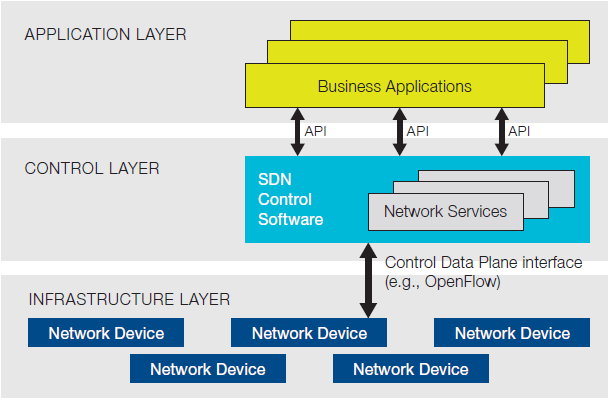
\includegraphics[scale=0.4]{Introduction/Image/SDNStructure.png}
\caption{\ac{SDN} structure}
\label{fig:sdn-and-openflow-overview:sdn-structure}
\end{figure}

The \ac{CP} is simply programmable with a higher level of abstraction and as result the network appears to application as a single point of exchange.
\ac{SDN} expected \ac{API} that allow the implementation of network services like: routing, multicast, security, access control, bandwidth management, traffic engineering, \ac{QoS} and energy management.

The communication between the \ac{CP} and the \ac{DP} occurs through the OpenFlow protocol. This protocol can be compared to a processor's instruction set and identify network flow based on rules that can be: static or dynamic, programmed by the \ac{CP} in real-time.

The benefit of an \ac{SDN} architecture based on OpenFlow are: (a) centralized control of multi vendor environments because each vendor can implement the algorithm as it sees fit but in respect with the OpenFlow standard interface multi vendor device can receive the same directive; (b) reduction of complexity through automation that derive from the previous point because when an user program the controller automatically the rules are applied on each devices; (c) high rate of innovation, (d) higher level of reliability and security and finally (e) more granular level of control of entire network architecture.

The OpenFlow switch is composed by one or more flow tables, a group table and a channel for the external controller.

A flow table contains a flow set composed by match fields, counters and instruction set apply to packet that match with fields.

When a packet arrives the devices try to match it with the flows present in the table and this control can be positive or negative. In case of positive match the instruction set are applied to the packet otherwise the action depend by the device configuration. It can forward the packet to the controller via the internal channel, can be dropped otherwise can be forward to the next flow table.

The instruction set can include operation which the forward of a packet, modify a field in the packet, group table processing (used for complex operation like multicast) and pipeline processing. In pipeline processing the packet is forwarded to a next flow table and with it the protocol can exchange some information in the form of meta data.

The network flows can be forwarded to a physical or virtual port (the virtual ports are used for internal management) or to a group table where are applied, to the packet, rules more complex like multicast or reroute fast.